\chapter{Rozbor řešené problematiky}
Tato kapitola v~úvodu popisuje několik existujících portálu. Dále přibližuje základní koncepcí vývoje webu a praktiky, které jsou při tomto vývoji často využívány. Následně jsou v~této kapitole popsány jazyky a knihovny, využívané při implementaci této bakalářské práce.

\section{Webové portály}
Webový portál je druh webové stránky, která shromažďuje informace z~vícero různých zdrojů a uživateli ty nejrelevantnější informace prezentuje uživateli shromážděné na jednom místě~\cite{bib:portal-liferay}.

Zpravidla je umožněno na portálu v~těchto informací vyhledávat. Velmi časté je také zakomponování autentizace uživatele a podle jeho role jsou mu zpřístupněny různé části daného portálu~\cite{bib:portal-indiana}.

% mozna vzit neco z https://books.google.cz/books?hl=cs&lr=&id=UMrhZfRpd8wC&oi=fnd&pg=PR6&dq=web+portals&ots=9bYmjTd1n2&sig=kw9YCnyaFh9n87y2VY05lITcZFc&redir_esc=y#v=onepage&q=web%20portals&f=false
\blindtext[2]

\subsection{CORDIS}
CORDIS\footnote{CORDIS: \url{https://cordis.europa.eu/}} (\emph{The Community Research and Development Information Service}) je portál provozovaný Evropskou Unií (dále jen EU) sloužící jako hlavní zdroj výsledků projektů, sponzorovaných v~rámci programů EU pro výzkum a inovaci. Na jednom místě veřejně poskytuje informace jak o~těchto projektech, tak i o~jejích účastnících, o~hlášeních, vědeckých zprávách a publikacích~\cite{bib:cordis}.
\blindtext

\subsection{The Funding \& Tenders Portal}

The Funding \& Tenders Portal\footnote{The Funding \& Tenders Portal: \url{https://ec.europa.eu/info/funding-tenders/opportunities/portal/screen/home}} je portál spravován převážně Evropskou komisí. Portál zprostředkovává informace určené hlavně expertům a účastníkům v~programech financovaných EU.
% https://ec.europa.eu/info/funding-tenders/opportunities/portal/screen/home 5.5.
V~případě zájmu o~zažádání financování výzkumu je nutné nejprve prostřednictvím toho portálu najít výzvu k~předkládání návrhů v~odpovídajícím odvětví a dodržet konkrétní postup pro podání žádosti.
% https://ec.europa.eu/info/funding-tenders/how-eu-funding-works/how-get-funding/find-funding-opportunity_en 5.5
\blindtext




\section{Vývoj webu}
\emph{Tato kapitola čerpá z~\cite{bib:web-development}}.

Tvorba webových stránek se obecně rozlišuje do dvou celků zvaných \emph{frontend} a \emph{backend}.

Frontendová část webu je to, co uživatel vidí, když stránku navštíví. Sestavení této části se v~žádném případě neobejde bez značkovacího jazyka HTML (\emph{Hypertext Markup Language}), který udává strukturu a obsah webové stránky. Další nedílnou součástí jsou kaskádové styly neboli CSS (\emph{Cascading Style Sheets}). Ty se starají o~to, jak bude obsah stránky esteticky působit. Další součástí, se kterou se setkáte téměř na každém webu je skriptovací jazyk JavaScript, který umožňuje webové stránky obohatit o~interaktivitu.
Zpracování této části webu probíhá v~klientovi - tedy internetovému prohlížeči uživatele. Na základě toto faktu se lze každé stránce na internetu \uv{nahlédnout pod pokličku} a zdrojové kódy frontendové části zobrazit, ve většině případů i rovnou v~internetovém prohlížeči upravit, což má samozřejmě vliv jen pro současného uživatele a ostatním návštěvníkům se tyto změnu neprojeví.

Oproti tomu backendová část je od uživatele izolována a zdrojové kódy pro něj nejsou přístupné, pokud je sám autor někde nezveřejní. Jejich interpretace totiž probíhá přímo na serveru a ten poté klientovi odešle již zpracovanou frontendovou část. Výběr technologie implementace backendové části je podstatně rozmanitější, patří mezi ně například Python, PHP, Java, C#, C++, .NET, Ruby a další. Díky prostředí Node.js\footnote{Node.js: \url{https://nodejs.org/en/}} lze ale využít i dříve zmiňovaný JavaScript, který sám o~sobě pro tento účel není primárně určen. 


\subsection{MVC architektura}
\emph{Tato kapitola čerpá z~\cite{bib:mvc}}.

Většinu aplikací lze obecně rozdělit na tři hlavní celky - data, rozhraní a logiku. V~anglickém jazyce se tyto celky dají nazvat pomocí slov \emph{model}, \emph{view} a \emph{controller} (zkratka MVC). Historie této architektury sahá až do sedmdesátých let, nicméně je v~dnešním světe stále naprostým standardem vývoje.

\begin{figure}[H]
	\centering
	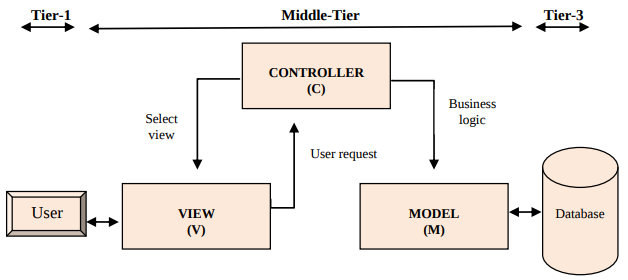
\includegraphics[width=\textwidth]{images/mvc.png}
	\caption{Diagram toku akcí při využití architektury MVC~\cite{bib:mvc}}
	\label{mvc}
\end{figure}

\begin{itemize}
\item Pojmem pohled (\emph{view}) se označuje uživatelské rozhraní (například stránka zobrazená v~prohlížeči), tato vrstva prezentuje data a je to také jediná vrstva, s~kterou uživatel přímo komunikuje. Akce provedené v~pohledu se předají kontroleru ke zpracovaní.
\item Kontroler (\emph{controller}) se chová jako prostředník mezi daty a rozhraním, zpracovává požadavky uživatele a provede s~modelem potřebné akce. Ve většině případu po provedené akci kontroler znovu obnoví pohled.
\item Model je obvykle objekt obsahující patřičná data z~databáze. Zprostředkovává jak jejich získání, tak i ukládání. Mimo to může být objekt obohacen i o~funkce, zpracovávající tyto data (například může převádět Unixový čas do formátu lépe čitelného pro člověka). 
\end{itemize}


Oddělením těchto celků je zajištěna lepší organizovanost zdrojových kódů a tím je usnadněn rychlejší vývoj. Jednotlivé celky jsou také lehčeji znovupoužitelné a práce programátorů na nich může probíhat souběžně. Rozdělením je také možné pro jeden pohled mít pohledů hned několik. Další pohledy mohou přibývat nebo naopak ty stávající mohou být smazány a na databázi aplikace to nebude mít žádný vliv.


\subsection{Responzivita}
\emph{Tato kapitola čerpá z~\cite{bib:responsive}}.

Před několika lety bylo zvykem tvořit webové stránky s~pevnou šířkou obsahu. Tato šířka byla volena tak, aby bylo možné stránku zobrazit jak na starších monitorech s~poměrem stran 4:3, tak i na modernějších širokoúhlých monitorech. 

Se stále rostoucí oblibou a dostupností chytrých telefonu ale přišel do hry nový hráč. Objevila se potřeba webové stránky uzpůsobit i pro tyto zařízení s~různorodou velikostí obrazovky. Webová stránka, která nenabízí responzivní design sice na mobilním zařízením lze zobrazit, ale prohlížení takové stránky není pro uživatele nikterak přívětivé. Uživatel může být nucen stránku neustále přibližovat a oddalovat, aby se dostal k~části, s~kterou zrovna potřebuje pracovat, nebo aby se mu podařilo stisknout konkretní tlačítko či odkaz. 

Díky nástupu nových verzí frontendových jazyků HTML5 a CSS3 je možné tuto situaci řešit bez nutnosti použití backendových řešení. Nejpřínosnější novinkou jsou tzv. \emph{media queries} v~kaskádových stylech, díky kterým je možné aplikovat odlišné styly na základě specifikací zobrazovacího zařízení. Jak již bylo v~úvodu zmíněno, design stránky se nejčastěji odvíjí od šířky obrazovky zařízení. V~souboru s~kaskádovými styly se tedy lze potkat například s~následující \emph{media query}.

\begin{verbatim}
    @media(max-width: 640px)
    {
        /* Specifické styly */
    }
\end{verbatim}

Takto obalené styly budou aplikovány jen v~případě, že zobrazovací zařízení splňuje podmínku v~kulatých závorkách. V~tomto případě se jedná o~zařízení s~šířkou obrazovky menší nebo rovnou 640 pixelům. Taková obrazovka může být ku příkladu moc malá na zobrazení postranního panelu s~navigací. Řešením takové situace v~drtivé většině případu bývá skrytí navigace do značně menšího tlačítka označujícího se jako \uv{hamburgerové menu} (anglicky \emph{hamburger menu}).

\begin{figure}[H]
	\centering
	
\includegraphics[width=0.5\textwidth-0.4cm]{images/fb-hamburger-1.png}
	\hspace{0.5cm}
	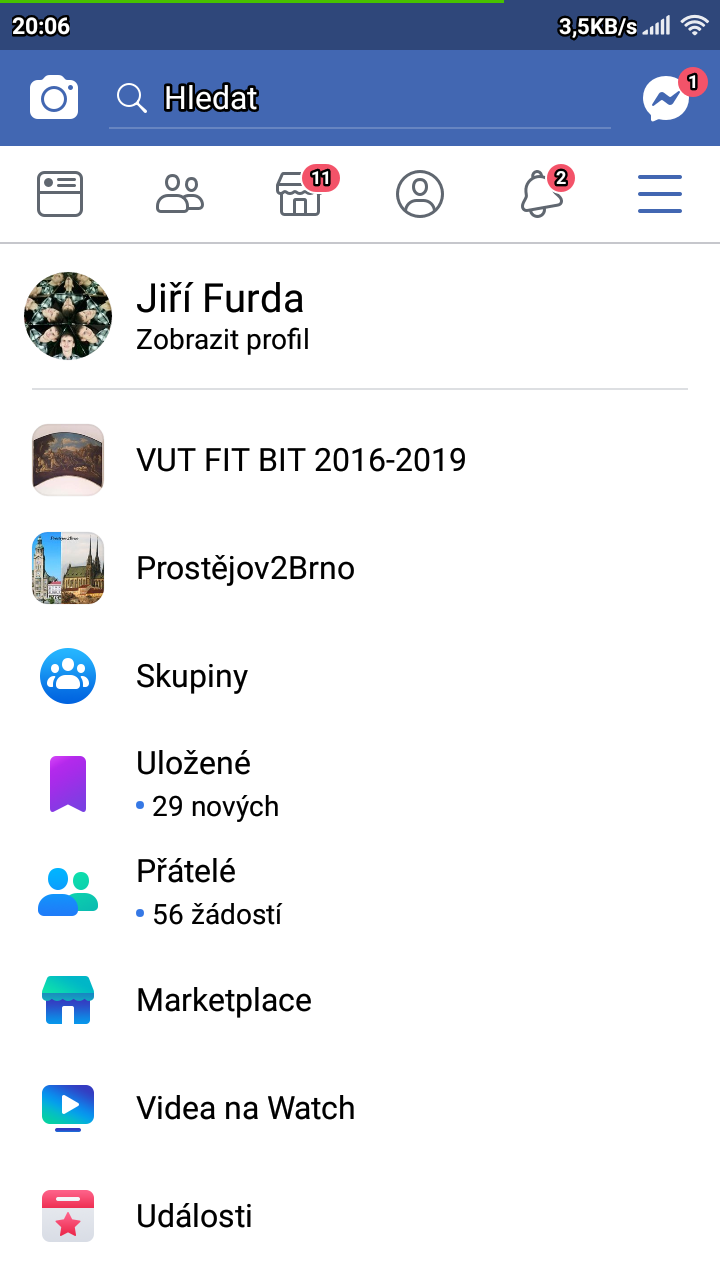
\includegraphics[width=0.5\textwidth-0.4cm]{images/fb-hamburger-2.png}
	\caption{Hamburgerové menu použité v~mobilní aplikaci sociální sítě Facebook\footnote{Mobílní aplikace Facebook v~obchodě Google Play: \url{https://play.google.com/store/apps/details?id=com.facebook.katana&hl=cs}}}
	%TODO zakryt jmeno
\end{figure}



\subsection{Princip nejdřív mobil}\label{section:mobile-first}
Ustálenou technikou, jak vyvíjet responzivní design webových stránek je princip \uv{nejdříve mobil} (anglicky \emph{mobile-first}). Jak název vypovídá, základní myšlenkou tohoto principu je nejdříve myslet na mobilní zařízení a až poté na desktopová zařízení. Tento přístup je možné aplikovat jak pro samotný návrh designu, tak i pro jeho následnou implementaci.

Protože mobilní zařízení nabízejí o~mnoho menší zobrazovací plochu než desktop, je zde každý kus prostoru drahocenný. Designér si proto musí nejprve ujasnit, které části webové stránky jsou pro uživatele prioritní a na základě těchto priorit sestavit návrh.

V~případě využití tohoto principu při samotné implementaci designu se postupuje obdobně. Pokud jsou všechny kaskádové styly jak pro mobilní, tak pro desktopová zařízení zapsána v~jednom souboru, bude tento soubor nejprve obsahovat styly společné pro obě tyto zařízení a styly určené pouze pro mobilní zařízení. Až po těchto stylech se budou v~soboru objevovat \emph{media queries} s~podmínkou \texttt{min-width}, které budou od určité šířky displeje aplikovat styly určené pro desktopová zařízení. Díky tomu bude samotný kód stylů zjednodušen. U~mobilních zařízení bývá zpravidla potřeba méně stylů a často lze využít některé z~výchozích vlastností daných prvků~\cite{bib:mobile-first}.


\section{Boostrap}
\emph{Tato kapitola čerpá z~\cite{bib:bootstrap}}.

Bootstrap\footnote{Bootstrap: \url{https://getbootstrap.com/}} je frontendový framework pro snadný vývoj webových stránek. Je vyvíjen společností Twitter\footnote{Twitter: \url{https://twitter.com/}}, která jej v~roce 2010 vydala jako otevřený software. Jen dva roky poté se Bootstrap stal nejoblíbenějším projektem na stránce GitHub\footnote{GitHub: \url{https://github.com/}}. Bootstrap se skládá převážně z~kaskádových stylů, ale interaktivní prvky využívají programovací jazyk JavaScript s~knihovnou jQuery\footnote{jQuery: \url{https://jquery.com/}}. Pro interaktivní část ale existují i další alternativy využívající například Vue.js\footnote{BootstrapVue: \url{https://bootstrap-vue.js.org/}}, React\footnote{React Bootstrap: \url{https://react-bootstrap.github.io/}} nebo Angular\footnote{NG Bootstrap: \url{https://ng-bootstrap.github.io/#/home/}}.

Bootstrap se drží moderních zásad jako princip \uv{nejdřív mobil} (uvedený v~kapitole \ref{section:mobile-first}) a nabízí snadnou možnost tvorby responzivního designu. Mimo to také nabízí možnost využít moderně působící vzhled základních HTML prvků jako jsou například vstupní pole formuláře nebo tlačítka. Bootstrap ale poskytuje i celou řadu nových předpřipravených komponent a to ku příkladu karty, modální okna, stránkování, informační hlášky a spoustu dalších.

Vzhledem ke své rozsáhlé komunitě lze nalézt mnoho dalších uživateli tvořených komponent nebo dokonce celých hotových šablon postavených na tomto frameworku. Jedna ze stránek určená pro sdílení takového obsahu ze nazývá Bootsnipp\footnote{Bootsnipp: \url{https://bootsnipp.com/}}.



\section{Python}
\blindtext[2]


\subsection{Flask}
Flask\footnote{Flask: \url{http://flask.pocoo.org/}} je open source webový micro-framework napsaný v~programovacím jazyce Python. Klíčový znak micro-frameworků je co nejmenší nebo i nulová závislost na externích knihovnách~\cite{bib:flask-doc}.
Flask si si klade za cíl udržet co nejjednodušší jádro, ale zároveň se soustředí na možnost tento základ jednoduše rozšířit~\cite{bib:flask-pym}.

Smyslem frameworku Flask je být základním kamenem pro jakoukoliv webovou aplikaci. Z~tohoto důvodu na rozdíl od ostatních frameworků neobsahuje žádnou abstrakci databázové vrstvy nebo knihovnu pro formuláře. Tohoto lze docílit použitím některého z~rozšíření~\cite{bib:flask-design}.

Ve svém základu využívá šablonovací jazyk Jinja2\footnote{Jinja2: \url{http://jinja.pocoo.org/}} zjednodušující udržení konzistentní struktury stránek. Poskytuje například dědičnost šablon nebo znovupoužitelné bloky a dokáže se vypořádat s~bezpečnostními útoky typu XSS (\emph{Cross Site Scripting})~\cite{bib:jinja}.
Druhou knihovnou, kterou framework Flask využívá je Werkzeug\footnote{Werkzeug: \url{https://pypi.org/project/Werkzeug/}} - jedna z~nejpokročilejších knihoven pro rozhraní brány webového serveru (WSGI neboli \emph{Web Server Gateway Interface}), které umožňuje webovou aplikaci provozovat nezávisle na technologii použité na serveru~\cite{bib:flask-pep}.

Tento framework využívá například sociální síť Pinterest\footnote{Pinterest: \url{https://cz.pinterest.com/}}~\cite{bib:flask-pinterest}
nebo síťová dopravní společnost Lyft\footnote{Lyft: \url{https://www.lyft.com/}}~\cite{bib:flask-lyft} 
(podobná službě Uber\footnote{Uber: \url{https://www.uber.com/cz/cs/}})



\section{Vue.js}\label{section:Vue.js}
V~dnešní době jsou webové prohlížeče stále schopnější a výkonnější. Díky tomu se stává trendem přenášet stále větší části webové aplikace ze serveru na stranu klienta. Toho je docíleno pomocí programovacího jazyku JavaScript. V~současné době se nejvíce využívá knihovna jQuery, %[Todo: najít zdroj]
ale začali se objevovat pokročilejší frameworky jako například React\footnote{React: \url{https://reactjs.org/}}, Angular\footnote{Angular: \url{https://angular.io/}} a v~neposlední řadě Vue.js\footnote{Vue.js: \url{https://vuejs.org/}}.

Vue.js je progresivní framework - přizpůsobuje se složitosti projektu. Podobně jako dříve zmiňovaný Flask se nejedná o~rozsáhlý framework, jehož části by jste vypínali, ale jedná se o~základní framework, který můžete dále rozšiřovat~\cite{bib:vue-progressive}.
Díky tomuto přístupu učební křivka není tak strmá, jako u~konkurenčních frameworků. Jediné, co člověku pro začátek práce s~frameworkem Vue.js stačí je být obeznámen s~jazyky HTML a JavaScript~\cite{bib:vue-curve}.

Jedna z~předností toto frameworku je jednoduchost obousměrné vazby dat. Tato vazba znamená, že hodnota proměnné v~jazyce JavaScript je synchronizována s~hodnotou v~objektovém modelu dokumentu (DOM neboli \emph{Document Object Model}) a to stejné platí i v~opačném směru~\cite{bib:vue-binding}.
V~praxi může být tato funkce využita například v~internetovém obchodě, kdy uživatel klikne na tlačítko \uv{Přidat do košíku}, které pouze rozšíří pole košíku o~další produkt. Bez jakéhokoliv dalšího úsilí komponenty, závislé na této proměnné zaznamenají změnu a automaticky provedou odpovídající akce - košík přepočítá celkový počet vybraného zboží, celkovou cenu nákupu, zlevní se cena daného produktu, při koupi dalších kusů apod. 


\subsection{Vue Router}
Mezi oficiálně podporované knihovny patří například Vue Router\footnote{VueRouter: \url{https://router.vuejs.org/}}, umožňující tvorbu jednostránkové aplikace, kdy se načte pouze jedná jediná stránka a pomocí jazyku JavaScript a asynchroniích požadavků se mění části obsahu webu. Server v~takovém případě slouží pouze jako úložiště dat a veškerou prezentaci se stará strana klienta~\cite{bib:vue-router}. %TODO obsahuje pekny ilustrace


\subsection{Vuex}
Dalším oficiálním rozšířením je Vuex, knihovna pro správu stavu. Pokud se v~aplikaci používá více komponent, které využívají stejnou proměnnou, brzy se zdrojový kód stává neudržitelným. 
V~tuto chvíli je vhodné využit knihovnu Vuex. Jejím účelem je udržovat centrální stav proměnných, které jsou sdíleny napříč různými komponentami v~aplikaci. Tohoto je docíleno díky dodržování návrhového vzoru jménem Flux~\cite{bib:vuex-doc}. 
%TODO: Reference na MVC -> WTF?


\subsubsection*{Návrhový vzor Flux}
\emph{Tato kapitola čerpá z~\cite{bib:vuex-guide}}.

Mezi základní pilíře návrhového vzoru Flux patří několik následujících pravidel, kterých se Vuex drží.

\begin{itemize}
    \item \textbf{Jediný zdroj pravdy.} Data, která jsou sdílena více komponentami jsou uložena na jednom místě - sklad (anglicky \emph{store}) a jsou oddělena od komponent, které jé využívají. Komponenty mohou stále mít svá lokální data, ale nesmějí mít svou kopií sdílených dat, ty se vždy musí číst ze skladu.
    \item \textbf{Data pouze ke čtení.} Komponenty nesmějí přímo upravovat data ve skladu. V~případě potřeby změny těchto dat sklad pouze informují a ten se sám o~postará o~provedení změny pomocí tzv. mutací (Reprezentovány uzlem \emph{Mutations} v~grafu \ref{img:vuex-dataflow}). Díky tomu se minimalizuje šance nepředpokládaných změn těchto dat a funkce, starající se o~tyto změny jsou jednodušeji dohledatelné.
    %TODO: AddToCart mutation example?
    \item \textbf{Změny dat jsou synchronní.} Asynchronní provádění operací mnohdy přináší spoustu výhod, v~tomto případě je ale vyžadováno mutace provádět synchronně kvůli odstranění závislosti na pořadí a načasování různých událostí.
\end{itemize}

\begin{figure}[H]
	\centering
	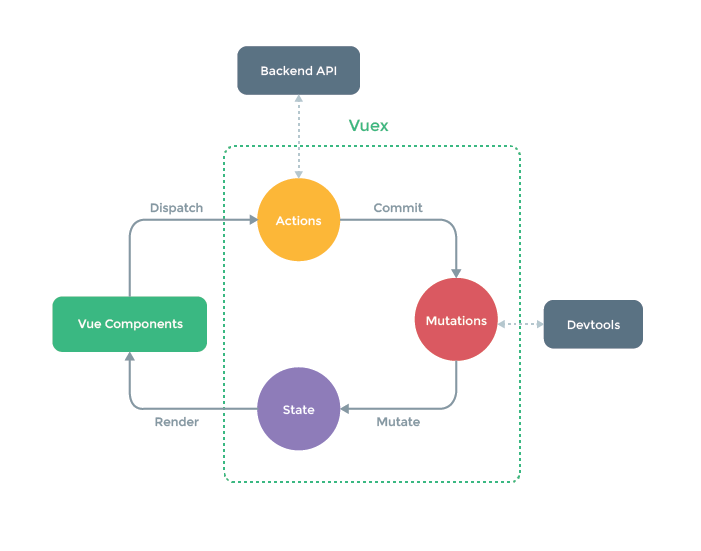
\includegraphics[width=\textwidth]{images/vuex.png}
	\caption{Diagram znázorňující životní cyklus dat v~knihovně Vuex~\cite{bib:vuex-doc}}
	%TODO: Popsat v obrázku nebo v textu?
	\label{img:vuex-dataflow}
\end{figure}

\blindtext


\subsubsection*{BootstrapVue}
\emph{Tato kapitola čerpá z~\cite{bib:bootstrap-vue}}.

BoostrapVue je frontendový framework založený na frameworku Boostrap, který pro svou plnou funkčnost vyžaduje použít také knihovnu jQuery. Pokud ale webová aplikace již pracuje s~frameworkem Vue.js, mnohdy odpadá potřeba jQuery v~aplikaci využívat. Vzhledem k~tomu, že se jedná o~poměrně rozsáhlou knihovnu, není žádoucí ji používat jen z~důvodu, že je aplikace postavená na frameworku Boostrap.

V~tuto chvíli je vhodné použít alternativu jménem BoostrapVue, která závislost na jQuery nahrazuje za závislost na Vue.js. Tento framework nabízí všechny komponenty původního frameworku, některé dokonce vylepšuje a také nabízí komponenty úplně nové.

Mimo to využití této knihovny také přináší větší pohodlí pro vývojáře. Dlouhý zápis některých komponent, tvořených pomocí množství vnořených prvků \texttt{<div>} lze díky Vue.js značně zjednodušit. Dokáže totiž prvek struktury HTML nahradit za rozsáhlejší strukturu na základě šablony komponenty. Konvencí frameworku je takové prvky pojmenovávat s~předponou \texttt{b-}, například tedy \texttt{b-button}.
Přímo učebnicovým příkladem takového zjednodušení je zápis modálního okna, které se klasickým způsobem tvoří následovně:

\begin{verbatim}
<div class="modal" tabindex="-1" role="dialog">
  <div class="modal-dialog" role="document">
    <div class="modal-content">
      <div class="modal-header">
        <h5 class="modal-title">Modal title</h5>
        <button type="button" class="close" data-dismiss="modal"
        aria-label="Close">
          <span aria-hidden="true">&times;</span>
        </button>
      </div>
      <div class="modal-body">
        <p>Modal body text goes here.</p>
      </div>
      <div class="modal-footer">
        <button type="button" class="btn btn-secondary"
        data-dismiss="modal">Close</button>
        <button type="button" class="btn btn-primary">Save changes</button>
      </div>
    </div>
  </div>
</div>
\end{verbatim}
\emph{Kód převzat z~\cite{bib:bootstrap-modal}}

Pomocí BoostrapVue lze identickou komponentu zapsat mnohem elegantnějším způsobem a to konrkétně:

\begin{verbatim}
<b-modal title="Modal title">
  <p>Modal body text goes here.</p>
</b-modal>
\end{verbatim}




\section{Elasticsearch}
\emph{Tato kapitola čerpá z~\cite{bib:elastic-defnitive}}.

Elasticsearch\footnote{Elasticsearch: \url{https://www.elastic.co/products/elasticsearch}} je volně šiřitelný vyhledávač umožňující distribuované vyhledávání a analýzu v~reálném čase. Umožňuje rychle pracovat s~rozsáhlými daty (anglicky \emph{big data}) a provádět nad nimi plnotextové vyhledávání, strukturované vyhledávání a nebo zmiňovanou analýzu.

Tento vyhledávač je hojně využíván jak menšími projekty, tak i světoznámými organizacemi. Za zmínku stojí například internetová encyklopedie Wikipedia\footnote{Wikipedia: \url{https://www.wikipedia.org/}}, britský deník The~Guardian\footnote{The Guardian: \url{https://www.theguardian.com/international}}, komunitní stránka pro výměnu rad programátorů StackOverflow\footnote{StackOverflow: \url{https://stackoverflow.com/}} nebo populární webová služba pro verzovací nástroj Git\footnote{Git: \url{https://git-scm.com/}} a to GitHub.

Elasticsearch je postavený nad knihovnou Apache Lucene\footnote{Apache Lucene: \url{https://lucene.apache.org/}}, využívá především její funkce plnotextového vyhledávání, ale oproti této knihovně samotné Elasticsearch nabízí o~mnoho přívětivější způsob používání, především pro začínající uživatele. 

Jedná se o~bezschémovou databázi, oproti relačním databázím nenabízí propojovací dotazy, a proto je nutné ukládaná data denormalizovat. Díky tomu jsou ale data a jejich metadata v~těsné blízkosti a tím je docíleno rychlé fulltextové vyhledávání~\cite{bib:elastic-what-is}.

\subsection{Základní struktura}
\emph{Tato kapitola čerpá z~\cite{bib:elastic-concept}}.

Základní struktura databáze Elasticsearch se na první pohled od tradičních relačních databázi velmi neliší, ke spoustě pojmů se dá najít ekvivalent.

\subsubsection*{Uzel a shluk}
Pod pojmem uzel (anglicky \emph{node}) se skrývá server, ve kterém jsou uložena data. Uzel v~rámci databáze může být jeden nebo jich může být i více a každý bude obsahovat pouze určitou část dat. Tyto uzly jsou seskupeny do shluku (anglicky \emph{cluster}).

\subsubsection*{Dokument}\label{section:dokument}
Dokument je základní jednotka dat, které může být zaindexována. Obsah dokumentu je zapsán ve formátu JSON (anglicky \emph{JavaScript Object Notation}). V~relační databázi lze dokument přirovnat k~řádku tabulky.

\subsubsection*{Index}\label{section:index}
Skupina dokumentů s~podobnou strukturou se nazývá index. Ekvivalentem v~relačních databázích by v~tomto případě byla tabulka.

\subsubsection*{Střepy}
Elasticsearch nabízí možnost index rozdělit na střepy (anglicky \emph{shards}), které mohou být uloženy v~různých uzlech. Tuto možnost je vhodné využít především při práci s~indexy s~velkým obsahem dat. Díky rozdělení docílíme distribuování zátěže a lze využít paralelní zpracování, tudíž bude zpracování dotazu odbaveno výrazně rychleji. 
Přístup k~takto rozděleným indexům se nijak nemění a pro uživatele je tento proces naprosto transparentní.

\subsubsection*{Repliky}
Obdobně lze využít i repliky. Zde se ovšem data indexu nerozdělují, ale naopak duplikují. Díky uložení těchto replik mezi více uzly může systém být robustnější a dokáže fungovat i v~případě selhání části shluku. I~v~tomto případě je umožněno vyhledávat paralelně. 

\subsection{Dotazy}
Pro komunikaci s~touto databází se využívá Query DSL - dotazy aplikačního rozhraní REST (anglicky \emph{Representational State Transfer}) ve formátu JSON.

Obsah dotazu může vypadat například následovně:
\begin{verbatim}
{
  "query": { 
    "bool": { 
      "should": [
        { "match": { "title": "Virtual Reality" }}, 
        { "match": { "title": "Augmented Reality" }}  
      ],
      "filter": [ 
        { "term":  { "participant.country.keyword": "Czech Republic" }}
      ]
    }
  }
}
\end{verbatim}

\blindtext

Na tento dotaz můžeme od serveru dostat odpověď s~obsahem:

\begin{verbatim}
{
  "took" : 38,
  "timed_out" : false,
  "_shards" : {
    "total" : 5,
    "successful" : 5,
    "skipped" : 0,
    "failed" : 0
  },
  "hits" : {
    "total" : 1515,
    "max_score" : 15.635861,
    "hits" : [
      {
        "_index" : "xstane34_projects",
        "_type" : "data",
        "_id" : "101785",
        "_score" : 15.635861,
        "_source" : {
          "startDate" : "2012-01-01",
          "endDate" : "2015-12-31",
          "reference" : "278169",
    ...
\end{verbatim}

\blindtext


\subsubsection*{Kontext}
Dotazy v~Elasticsearch se rozlišují na dva základní typy - kontext dotazu (\emph{query}) a kontext filtru.
První z~nich se dá lidsky přeložit do otázky \uv{Jak moc dokument splňuje dotaz?}. V~tomto případě se u~každého výsledku počítá skóre relevance, podle kterého jsou ve výsledné odpovědi dokumenty sestupně řazeny.

\subsection{Metadata}
\blindtext

\subsection{Fasetové vyhledávání}
S~velkým množstvím dat přichází potřeba obsah podle určitých kriterií zúžit. K~tomutu účelu slouží filtry a fasetové vyhledávání (někdy také označována jako fastová navigace - anglicky \emph{faceted search} nebo \emph{faceted navigation}). Využití faset je ale pokročilejší než použít filtry, protože fasetová navigace umožňuje využít hned několik filtrů najednou~\cite{bib:facet}.

V~Elasticsearch je možné tuto navigaci vytvořit pomocí tzv. kyblíkových agreagací (angl. \emph{bucket aggregations}).
Jednoduše řečeno, se pro dokumenty vytvoří kyblíky, kde každý z~kyblíku odpovídá určitému kriteriu. Pokud dokument toto kriterium splňuje, je do kyblíku vložen~\cite{bib:elastic-bucket}.

S~tímto typem vyhledávání se lze setkat velmi často v~seznamech produktů například v~internetových obchodech nebo cenových srovnávačích.

\begin{figure}[H]
	\centering
	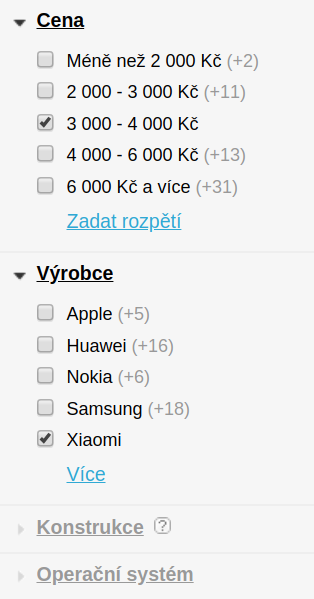
\includegraphics[width=0.35\textwidth]{images/heureka-facet.png}
	\caption{Příklad využití fasetového vyhledávání na cenovém srovnávači Heureka\footnote{Heureka: \url{https://www.heureka.cz/}}}
\end{figure}


\subsection{Plnotextové vyhledávání}
\emph{Tato kapitola čerpá z~\cite{bib:elastic-defnitive}}.

Uložená data se dělí na dva typy - přesné hodnoty a plnotextové hodnoty (anglicky \emph{full-text}). Přesné hodnoty jsou určeny pro data, jako například identifikátor uživatele. Pokud totiž vyhledáváme uživatele s~identifikátorem \uv{42}, jako výsledek neočekáváme uživatele, který má identifikátor \uv{420}, ale očekáváme výsledek, který bude přesně splňovat hledanou položku.
Pokud ale člověk pracuje s~textovými položkami, nemusí nutně hledat stoprocentní shodu. Lidský jazyk je velice rozmanitý a umožňuje slova časovat, skloňovat, či vyjádřit jednu věc vícero synonyma. %todo sklonuju spravne?
V~těchto případech hledání totožných hodnot selhává, i když má text z~pohledu člověka stejný nebo podobný význam. Pro tento typ hledání slouží právě plnotextové hledání. Můžeme se s~ním setkat například při hledání článku v~internetovém magazínu.
Elasticsearch pro takové hledání musí text nejprve analyzovat a vytvořit pro něj obrácené indexy.

\subsubsection*{Obrácený index}
Obrácený index (anglicky \emph{inverted index}) je struktura obsahující seznam všech unikátních slov vyskytujících se v~uložených dokumentech. Pro každé z~těchto slov uchovává informaci, ve kterých dokumentech se vyskytovalo. Díky tomu je možné v~textových položkách rychle provádět plnotextové hledání.

Příkladem mohou být dva dokumenty, kde každý obsahuje právě jednu z~následujících vět:
\begin{itemize}
    \item TODO
    \item TODO
\end{itemize}
Zpracování těchto dokumentů tedy může vzniknout následující obrácený index:

TODO table

Takovýto index by byl ale v~praxi nepoužitelný. Text nestačí pouze strojově rozdělit do tokenů, ale musí proběhnout celá analýza textu.

\subsubsection*{Analýza}
Analýza představuje proces, kdy se kus textu rozdělí do jednotlivých tokenů a následně se tyto tokeny upraví do podoby vhodné pro použití plnotextového vyhledávání. Tento proces obstarává analyzér, který se skládá ze tří části:
\begin{itemize}
    \item \emph{Filtry znaků} upraví zpracovávaný řetězec ještě před samotným rozdělením do tokenů. Jeho úkolem může například být odstranění HTML značek z~textu.
    \item \emph{Tokenizér} z~textu sestaví jednotlivé tokeny. Tokeny ve většině případů představují jednotlivá slova, ale nemusí tomu tak vždy být. 
    \item \emph{Filtry tokenů} na konec projde všechny vytvořené tokeny, může některé odstranit, přidat a nebo jen upravit. 
\end{itemize}
Filtrů může být v~jednom analyzéru použitá celá řada a to jak filtrů znaků, tak i filtrů tokenů. Tokenizér je ale v~rámci analyzéru vždy použit jen jeden jediný.

Elasticsearch již ve svém základu nabízí škálu různých analyzéru. Tyto analyzéry jsou různé složitosti, mezi ty nejjednodušší patří analyzér bílých znaků, který text rozdělí striktně podle mezer, tudíž je i tečka na konci věty vnímána jako část slova. Nejčastěji se ale člověk může setkat s~jazykovým analyzérem, který je uzpůsoben lidské řeči. Elasticsearch takový analyzér nabízí pro mnoho jazyků mezi které patří i jazyk český.

\subsubsection*{Filtry tokenů}
\emph{Tato kapitola čerpá z~\cite{bib:elastic-fulltext}}.

Velmi častou filtrací bývá změna velkých písmen na malé, díky tomu nejsou slova na začátku věty vnímána jako jiná slova, než ty v~jiné části věty. Pro český jazyk je také typické odstranění diakritiky.

Součástí analyzátorů bývá často odstranění tokenů, které obsahují nepodstatná slova. Jedná se především o~spojky a předložky. Taková slova se v~plnotextovém vyhledávání označují jako \emph{stop slova} (anglicky \emph{stop words}). Tento seznam je vždy specifický pro konkrétní jazyk textu, použít výchozí anglická stop slova nad česky psaným textem by ztrácelo význam.

Další nedílnou součástí pokročilejších analyzátorů je \emph{stematizace}, aneb získání kmene slova. Pro tuto operaci lze využit dva způsoby a to algoritmus nebo slovník. Každý z~těchto způsobů má své pro a proti.
Využitím algoritmické stematizace sice analyzátor nemusí znát všechna slova v~daném jazyce, protože slova převádí do požadovaného tvaru pouze na základě sady pravidel, ale zase dochází k~určité nepřesnosti. Elasticsearch v~případě využití české algoritmické stematizace ze slov odstraňuje všechny přípony.
Druhým způsobem, který lze využít je stematizace na základě slovníku. Díky tomu jsou převedené tvary přesnější než ty získané algoritmem, ale hlavním předpokladem je využití vhodného slovníku s~dostatečnou zásobou slov.
%TODO priklad

\subsection{Podobnostní hledání}
\blindtext[2]

\subsection{Knihovny}
Elasticsearch také vyvíjí několik oficiálně podporovaných nízkoúrovňových klientů pro mnoho populárních programovacích jazyků. Patří mezi ně například Java, JavaScript, Go, .NET, PHP, Perl nebo Python~\cite{bib:elastic-clients}.
Klientů vyvíjených komunitou lze samozřejmě nalézt o~mnoho více\footnote{Komunitní klienti Elasticsearch: \url{https://www.elastic.co/guide/en/elasticsearch/client/community/current/index.html}}.

Práce s~nízkoúrovňovými klienty pro programátory nebývá příliš pohodlná, z~tohoto důvodu vznikají komunitou vyvíjení klienti, kteří nabízí vysokoúrovňový přístup. Konkrétně pro programovací jazyk Python byl do roku 2015 společností Mozilla\footnote{Mozzila: \url{https://www.mozilla.org/}} vyvíjen klient jménem \emph{ElasticUtils}\footnote{ElasticUtils: \url{https://elasticutils.readthedocs.io/en/latest/}}. Za nástupce toho klienta je považována knihovna \emph{Elasticsearch DSL}~\cite{bib:elastic-utils}.

\subsubsection*{Elasticsearch DSL}
\emph{Tato kapitola čerpá z~\cite{bib:elastic-dsl}}.

Elasticsearch DSL je rovněž knihovna pro programovací jazyk Python. Jedná se o~vysokoúrovňovou knihovnu postavenou na oficiální nízkoúrovňové knihovně \texttt{elasticsearch-py}. Díky tomu lze s~dokumenty v~databázi Elasticsearch pracovat jako s~objekty, ale zároveň je stále možné použít původní přístup oficiálního klienta  ku příkladu ke zjištění zdraví shluku.

Jako příklad mějme následující dotaz, napsaný s~využitím oficiální knihovny \texttt{elasticsearch-py}.
\begin{verbatim}
from elasticsearch import Elasticsearch
client = Elasticsearch()

response = client.search(
{
  index="xstane34_projects",
  body={
    "query": { 
      "bool": { "must": { "title": "Virtual Reality" }}, 
        "filter": [ 
          { "term":  { "participant.country.keyword": "Czech Republic" }}
        ]
      }
    },
    "aggs": {
        "coordinator_coutry": {
          "terms": {"field": "coordinator.country.keyword"},
        }
      }
  }
\end{verbatim}

Tento poměrně zdlouhavý dotaz lze se stejným výsledkem přepsat za použití knihovny Elasticsearch DSL do následující formy:

\begin{verbatim}
from elasticsearch import Elasticsearch
from elasticsearch_dsl import Search

client = Elasticsearch()

s~= Search(using=client, index="xstane34_projects")  \
    .query("match", title="Virtual Reality")  \
    .filter("term", coordinator__country__keyword="Czech Republic")

s.aggs.bucket("coordinator_coutry", "terms",  \
    field="coordinator.country.keyword")

response = s.execute()
\end{verbatim}
%TODO zkontrolovat

\blindtext[2]